\section{问题四：定向干扰源的搜索、定位与清除}
\label{new:sec-q4}

\subsection{问题特征与建模思路}

问题四与问题三的根本差别不在于接收距离，而在于信号具有方向性。设源位置为 $g$，单位发射法向为 $n$，机器人在 $p$ 处检测；除距离条件 $\norm{p-g}\le1000$ 外，还需满足
\begin{equation}
 n^{\mathsf T}(p-g)\ge0.
 \label{q4:eq-front}
\end{equation}
因此，距离覆盖并不能推出可探测性：位于源附近但处于其发射背面的点，可能完全没有信号。特别是源在圆域边界且朝外发射时，圆内的近邻点都可能落在背向半平面。问题三的七点环只证明每个源附近存在一个距离足够小的点，不能保证式 \eqref{q4:eq-front}，所以问题四必须同时覆盖位置和方向。

我们采用“先建立方向鲁棒发现骨架，再对已发现频道局部定位”的两层结构。第一层不依赖在线知道 $g$ 或 $n$，只要求所有可能源位置和所有发射方向均有一个安全检测点；第二层使用实际测向反馈逐步收缩可行域，并在接收成功后完成清除。这样，搜索保证与局部效率分开，任何扫描排序都不会改变覆盖证书。该“覆盖保证—路径规划”分层也与无人系统区域覆盖研究中的建模思路一致\cite{jia}。

\begin{figure}[htbp]
\centering
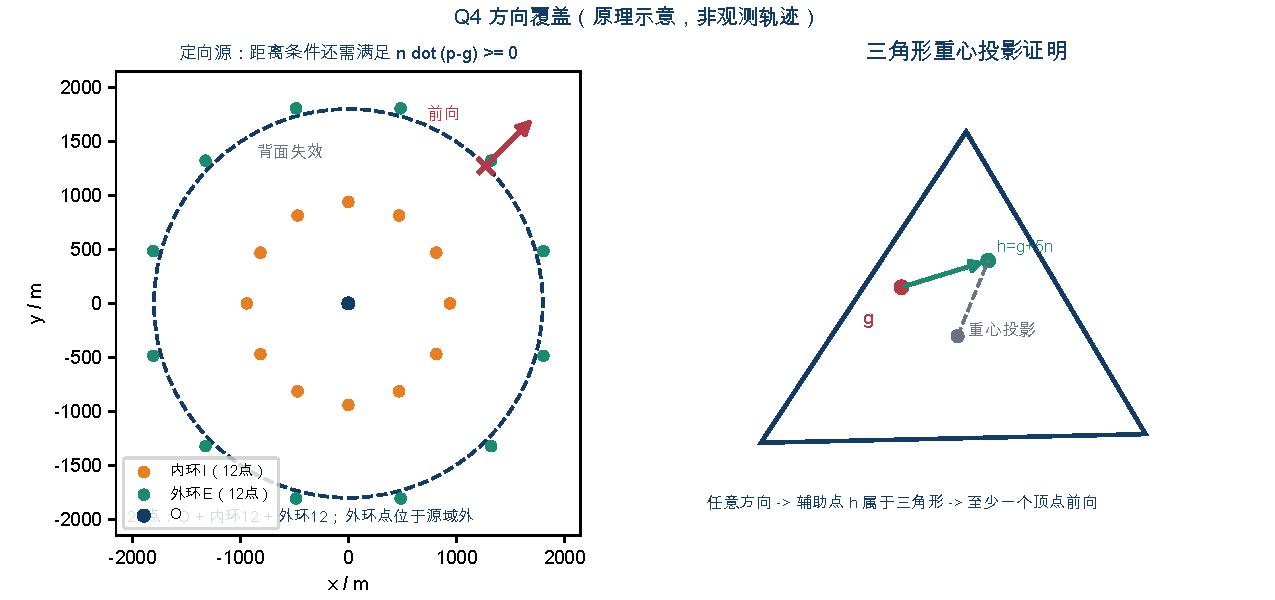
\includegraphics[width=0.92\textwidth]{figures/competition_direction.pdf}
\caption{25点错相双环的方向覆盖示意。外环点位于源域外，辅助点 $h=g+5n$ 仅用于证明，不表示观测轨迹；图中几何关系为示意图。}
\label{q4:fig-direction}
\end{figure}

\subsection{25点错相双环发现骨架}

取 $a=940$ m、$b=1870$ m，令 $u(\theta)=(\cos\theta,\sin\theta)$，布置原点、内环12点和外环12点：
\begin{equation}
\begin{aligned}
 p_0&=O=(0,0),\\
 I_k&=a u(k\pi/6),\qquad k=0,\ldots,11,\\
 E_k&=b u(k\pi/6+\pi/12),\qquad k=0,\ldots,11.
\end{aligned}
\label{q4:eq-skeleton}
\end{equation}
内环相邻点相差 $30^\circ$，外环相对内环错开 $15^\circ$。13个点位于源圆域内，12个点位于圆域外；外部点不是多余的行程点，而是为方向覆盖提供前方候选。点的编号只表示扫描义务，不规定实际访问顺序。

将下标按模12计算，外正十二边形由 $E_k$ 的凸包给出。其内部由36个闭三角形剖分：
\begin{equation}
\begin{aligned}
 T_k^{(1)}&=\conv\{O,I_k,I_{k+1}\},\\
 T_k^{(2)}&=\conv\{I_k,E_k,I_{k+1}\},\\
 T_k^{(3)}&=\conv\{I_{k+1},E_k,E_{k+1}\},
 \end{aligned}
\qquad k=0,\ldots,11.
\label{q4:eq-triangles}
\end{equation}
第一类填充内十二边形，后两类填充内外两环之间的带状区域。由于外环相对内环错开半个扇区，连接边在各个 $15^\circ$ 扇区内不交叉；且 $a<b\cos(\pi/12)$，内环点严格位于相应外边的内侧。因此这些闭三角形没有孔洞，覆盖整个外正十二边形。

记 $c=\cos(\pi/12)$、$s=\sin(\pi/12)$。三角形边长只有四类：
\begin{equation}
 \ell_0=a,\qquad \ell_I=2as,\qquad \ell_E=2bs,\qquad
 \ell_{IE}=\sqrt{a^2+b^2-2ab c}.
 \label{q4:eq-lengths}
\end{equation}
由 $c>0.9659$、$0.25<s<0.259$ 得
\begin{equation}
 bc>1805,\qquad
 \ell_0<993,\quad \ell_I<486.92,\quad \ell_E<968.66,
 \quad \ell_{IE}<993.
 \label{q4:eq-bounds}
\end{equation}
故每个三角形的直径 $D_T<993$ m，同时外十二边形包含半径1805 m的圆盘 $B(O,1805)$。前一个界控制候选点到三角形内辅助位置的距离，后一个界保证辅助位置仍在剖分覆盖范围内。

\subsection{方向覆盖的关键证明}

\begin{theorem}[25点的方向鲁棒覆盖]\label{new:thm-direction-cover}
对任意 $g\in\disk$ 和任意单位向量 $n$，式 \eqref{q4:eq-skeleton} 至少存在一个顶点 $v$，使得理想点和总位置误差不超过1 m的实际点 $v'$ 满足
\begin{equation}
 n^{\mathsf T}(v'-g)\ge4\ {\rm m},\qquad \norm{v'-g}<999\ {\rm m}.
 \label{q4:eq-direction-margin}
\end{equation}
\end{theorem}

\begin{proof}
引入仅用于证明的辅助点
\begin{equation}
 h=g+5n.
 \label{q4:eq-helper}
\end{equation}
由于 $\norm g\le1800$ 且 $\norm n=1$，有 $\norm h\le1805$，从而 $h$ 落在外十二边形内，必属于至少一个闭三角形 $T$。将其写成该三角形三个顶点的重心组合 $h=\sum_{i=1}^3\lambda_i v_i$，其中 $\lambda_i\ge0$ 且 $\sum_i\lambda_i=1$。线性投影给出
\begin{equation}
 \sum_{i=1}^3\lambda_i n^{\mathsf T}(v_i-g)
 =n^{\mathsf T}(h-g)=5.
 \label{q4:eq-projection}
\end{equation}
因此至少有一个正权重顶点 $v$ 满足 $n^{\mathsf T}(v-g)\ge5$。同时 $v,h$ 同在 $T$ 中，故
\begin{equation}
 \norm{v-g}\le \norm{v-h}+\norm{h-g}\le D_T+5<998.
 \label{q4:eq-distance}
\end{equation}
若实际检测点满足 $\norm{v'-v}\le1$，柯西不等式和三角不等式分别给出
\[
 n^{\mathsf T}(v'-g)\ge5-1=4,
 \qquad \norm{v'-g}<998+1=999.
\]
这同时保证严格位于发射前方和最小接收圆盘内。\end{proof}

证明中的 $h$ 是方向覆盖的等价转换：任意方向只需把源沿发射方向平移5 m，再由有限三角形剖分找到一个顶点。它不代表机器人实际访问的位置，也不需要算法估计方向。源在圆周、辅助点落在边界、重心系数为零等退化情形均由闭三角形包含。1 m 是坐标计算、舍入和实际停靠误差的总预算，不可在不同误差来源间重复使用。

\subsection{有限可行路线与扫描执行}

25点骨架只要求每个点完成一次必要检测，访问顺序则交给有限路线组合。作为明确可行的开放路线，可按
\[
 O,I_0,I_1,\ldots,I_{11},E_{11},E_{10},\ldots,E_0
\]
访问全部点，其长度为
\begin{equation}
 L_{25}=a+22(a+b)\sin(\pi/12)
 +\sqrt{a^2+b^2-2ab\cos(\pi/12)}.
 \label{q4:eq-route}
\end{equation}
这是一条有限的开放可行路线；实际访问顺序还需结合频道清除、换频和局部定位反馈动态确定。

实际执行采用有限路线组合。对每个未完成骨架任务和已发现未清除频道建立代理任务：骨架点半径取0，已知频道取其当前可行域最小包围圆中心 $z_c$ 及半径 $r_c$。从当前位置 $q$ 出发，用
\begin{equation}
 J_\gamma(\pi)=\norm{q-z_{\pi_1}}+
 \sum_{j=1}^{n-1}\norm{z_{\pi_{j+1}}-z_{\pi_j}}
 +\gamma r_{\pi_1},\qquad \gamma=1
 \label{q4:eq-route-proxy}
\end{equation}
选择有限候选排列，保留最近插入、受限2-opt、Or-opt1以及两种不同首任务的近邻初解；最多进行 $\min(n,12)$ 轮最佳改善。每次只执行排列首项，执行后依据真实反馈重建任务集。所有操作均保持完整任务排列，联合调度只改变顺序，不删除方向覆盖所需的25个检测义务。

扫描频道采用 \texttt{useful} 规则：未知频道在每一个尚未完成的骨架点都必须检测；已有轨迹的频道仅当 $r_c>19.9$ 且 $\norm{p-z_c}-r_c\le1500$ m 时补测，否则跳过。边界等号属于“有用”一侧。这个判据只表达保守区域可能与接收范围相交，不保证定向源正面可见，因此不能把跳过检测当作负证据。已发现频道最终仍需收到清除成功反馈。

\subsection{局部定位、失信号恢复与光学兜底}

骨架检测或共享观测得到正信号后，沿用有限局部测向过程。对每个频道，只有在当前包围圆半径 $r_c>38$ m 且可能进入接收范围、并且此前未在完全相同坐标执行过预检测时，才至多执行一次原地 $\texttt{premeasure}$；该动作位于六次固定测向预算之外。预检测支付检测和换频费用，但不增加移动，也不保证定向源响应。

每次有效测向按返回的方向和距离约束收缩可行域。若下一次测向暂时失去信号，则：(1) 保留最近一次有效正测点 $s$ 作为恢复基准；(2) 在其方向轴上按既有反射/收缩规则生成下一个候选点；(3) 重新检测，并在获得新正信号后用新的 $s$ 更新轴。恢复点不把失败点与1500 m作平均。固定测向至多六次；若仍未获得成功清除，依次执行矩形光学兜底：以正测点和方向约束形成的可行域构造保守矩形，以半径19.9 m的蛇形覆盖逐点访问候选中心，并在每个候选处复核全部可行域顶点；收到 \texttt{success} 立即停止该频道。

对问题四，\textbf{正面规则是：定向源的无信号反馈只表示当前姿态下未收到信号，不能删去其1000 m位置圆盘；因此禁用负圆盘推断，并关闭 \texttt{approach\_clear}。} 可行域始终保留正观测约束及题设先验。矩形覆盖是对仍可能包含真源的区域进行有限穷举，不依赖对失信号原因的额外判断。

\subsection{停止条件、成本与有限终止}

令 $V=\{0,\ldots,24\}$ 为完整骨架索引集，$V_c$ 为频道 $c$ 已接受的实际骨架检测位置。频道证书定义为
\begin{equation}
 \operatorname{Cert}_c=
 \begin{cases}
 C,&\text{收到频道 $c$ 的成功清除反馈},\\
 N,&\text{从未发现该频道且全部 $V$ 上有效检测均无信号},\\
 U\text{ 或 }D,&\text{尚未确定或已发现但未清除}.
 \end{cases}
 \label{q4:eq-stop-cert}
\end{equation}
当未知频道完成全部25点且全无信号时，定理 \ref{new:thm-direction-cover} 排除了其存在，故可记为 $N$；一旦频道进入 $D$，只能通过成功清除转为 $C$，不能再改判无源。合法停止为
\begin{equation}
 \left[\forall c\in\{1,\ldots,20\},\ \operatorname{Cert}_c\in\{C,N\}\right]
 \quad\text{或}\quad
 \left[\#\{c:\operatorname{Cert}_c=C\}=16\right].
\end{equation}
第二项统计16个不同频道的成功清除；队列为空或长时间未发现新源都不是停止理由。

成本由实际移动、检测、清除、换频和光学尝试共同计入式 \eqref{eq:time}；25点骨架相对31点方案少120次潜在频道检测，但提前清除、\texttt{useful}跳过、预检测和局部定位会改变实际次数。路线组合的距离矩阵为 $O(n^2)$，有限插入与局部交换搜索为 $O(n^3)$；它们只用于产生可控的候选顺序，不改变覆盖保证。每个正常局部任务至多一次预检测、六次测向，随后成功清除或进入有限矩形覆盖；完整骨架只有25个点，最多处理16个真实源。因此在接口正常、误差预算成立且不被现实期限中断时，搜索、定位、清除和停止均在有限动作内完成。Q4的运行结果与成本由后续“模型检验”章节统一报告，本章不单列独立实验数字。
